% Drawing 144/08-5 -- folder 144, batch 08, archive page 155 (PDF page 156).
% Transcription: un petit cercle d'où partent trois segments ; entre deux d'entre eux, un secteur hachuré.
% Kind: small circle with three segments and a hatched sector. Method 2 (schematic redraw from the facsimile). Status: ok.
% Notes: Three segments leave the circle; the sector between the two right-hand ones is hatched.
% Coordinates: 1 unit = 1 mm = 1/100 of the crop width (bbox in page fractions: [0.12, 0.42, 0.28, 0.5]).
% Redrawn by Claude (claude-opus-5-5), issue #73, 2026-11-07; not checked by a human; not compiled (no TeX in the session).
% Rights: reproduces part of the work -- behind RENDER_TRANSCRIPTS, never published by itself.
\documentclass[tikz,border=3pt]{standalone}
\usepackage{amsmath,amssymb}
\usetikzlibrary{patterns,arrows.meta}
\tikzset{pencil/.style={black!45}, struck/.style={black!35}, mark/.style={circle,draw,inner sep=1.3pt}, pt/.style={circle,fill,inner sep=0.9pt}, opt/.style={circle,draw,fill=white,inner sep=1.1pt}}
\begin{document}
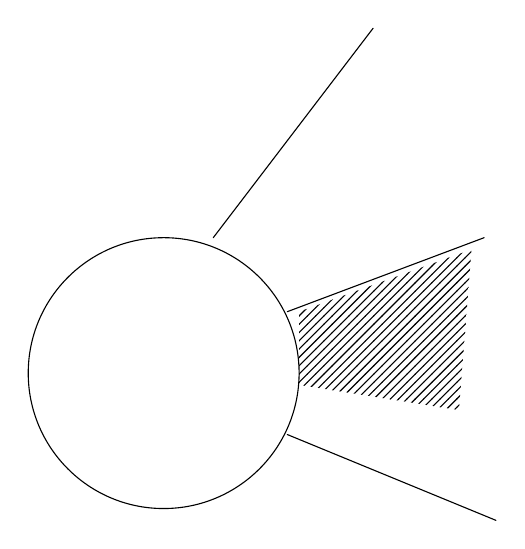
\begin{tikzpicture}[x=1mm,y=1mm,line cap=round,line join=round,font=\scriptsize]
\draw (35.9,-47.5) circle[radius=17.2];
\draw (42.2,-30.3) -- (62.5,-3.7);
\draw (51.6,-39.7) -- (76.6,-30.3);
\draw (51.6,-55.3) -- (78.1,-66.2);
\fill[pattern=north east lines] (53.1,-39.7) -- (75,-31.8) -- (73.4,-52.2) -- (53.1,-49) -- cycle;
\end{tikzpicture}
\end{document}
